\documentclass[10pt]{oblivoir}

\usepackage{fapapersize}
\usefastocksize{210mm,297mm}
\usefapapersize{190mm,260mm,20mm,20mm,35mm,35mm} 
\usepackage{mathtools}
\usepackage{amsthm}
\usepackage{amssymb}
\usepackage{tikz}
\usepackage{pgf,pgfplots}
\pgfplotsset{compat=1.15}
\usepackage{mathrsfs}
\usetikzlibrary{arrows}
\usepackage{lipsum}
\usepackage{jiwonlipsum}
\usepackage{tabularray}

\setsecnumformat{\csname the#1\endcsname.\quad}


%\linespread{1.0} % 영어 논문의 경우 줄간격 조절

%%%%%%%%%%%%%%%%%%%%%%%%%%%%%%%%%%%%%%%%%%%%%%%%%%%%%%%%%%%%%%%%%%%%
%-- 논문 주요 정보 표기
%%%%%%%%%%%%%%%%%%%%%%%%%%%%%%%%%%%%%%%%%%%%%%%%%%%%%%%%%%%%%%%%%%%%

\def\mytitle{English Title} % todo: English Title 를 지우고, 자신의 영문 연구 제목을 쓰시오.
\def\mytitleko{이것이 나의 연구 제목이다}  %todo: 이것이 나의 연구 제목이다 를 지우고 자신의 국문 제목을 쓰시오. 
 

\def\myauthorfirst{Hong Gildong1} %todo: Hong Gildong1 을 지우고 저자1의 영문 이름을 쓰시오.
\def\myauthorsecond{Hong Gildong2} %todo: Hong Gildong2 을 지우고 저자2의 영문 이름을 쓰시오.
\def\myauthorthird{Hong Gildong3} %todo: Hong Gildong3 을 지우고 저자1의 영문 이름을 쓰시오.
\def\myauthorfourth{Hong Gildong4} %todo: Hong Gildong4 을 지우고 저자2의 영문 이름을 쓰시오.

\def\myauthorfirstko{홍길동1} %todo: 홍길동1을 지우고 자신의 이름을 쓰시오.
\def\myauthorsecondko{홍길동2} %todo: 홍길동2를 지우고 자신의 이름을 쓰시오.
\def\myauthorthirdko{홍길동3} %todo: 홍길동3을 지우고 자신의 이름을 쓰시오.
\def\myauthorfourthko{홍길동4} %todo: 홍길동4를 지우고 자신의 이름을 쓰시오.

\def\affiliation{Sejong Academy of Science and Arts}
\def\affiliationko{세종과학예술영재학교}
\def\address{265, Dalbit 1-ro, Sejong-si, Republic of Korea}

\def\mykeywords{keyword1, keyword2, keyword3} %todo: 키워드 입력 (영문) 
\def\mykeywordsko{주요어1, 주요어2} %todo: 국문 주요어 입력
%%%%%%%%%%%%%%%%%%%%%%%%%%%%%%%%%%%%%%%%%%%%%%%%%%%%%%%%%%%%%%%%%%%%
%-- 논문 주요 정보 표기 끝
%%%%%%%%%%%%%%%%%%%%%%%%%%%%%%%%%%%%%%%%%%%%%%%%%%%%%%%%%%%%%%%%%%%%

\usepackage{caption}
\captionsetup[figure]{%
labelsep=period,
labelfont=bf, 
name={Figure}
}
\captionsetup[table]{%
labelsep=period,
labelfont=bf,
name={Table}
}


%%%%%%%%%%%%%%%%%%%%%%%%%%%%%%%%%%%%%%%%%%%%%%%%%%%%%%%%
%-- 정리류 환경 설정
\newtheorem{theorem}{\bfseries\sffamily 정리}[section]
\newtheorem{lemma}[theorem]{도움정리}
\newtheorem{corollary}[theorem]{따름정리}
\theoremstyle{definition}
\newtheorem{definition}[theorem]{정의}
\newtheorem{example}[theorem]{보기}
\theoremstyle{remark}
\newtheorem{remark}[theorem]{참고}

\numberwithin{equation}{section}
\renewcommand*{\proofname}{증명}

%==
% \renewcommand\qedsymbol{
% \hfill\ensuremath{\blacksquare}
%} 
%====
%-- 정리류 환경 설정 끝
%%%%%%%%%%%%%%%%%%%%%%%%%%%%%%%%%%%%%%%%%%%%%%%%%%%%%%%%%%%%%%

%---- description label 변경
% \renewcommand*\descriptionlabel
% [1]{\hspace\labelsep
% \scshape\mdseries #1}
%---------- description label 변경 끝

\newcommand{\splitatcommas}[1]{%
  \begingroup
  \begingroup\lccode`~=`, \lowercase{\endgroup
    \edef~{\mathchar\the\mathcode`, \penalty0 \noexpand\hspace{0pt plus 1em}}%
  }\mathcode`,="8000 #1%
  \endgroup
}



\usepackage{tikz}
\usetikzlibrary{calc,decorations.pathmorphing,shapes,patterns}
\newcommand{\checkerboard}[2]{
	\foreach \x  in {0,...,#1}{
   \draw (.5*\x  ,0 ) -- ++(0,.5*#2);
        }
\foreach \y  in {0,...,#2}{
   \draw (0  ,.5*\y ) -- ++(.5*#1,0);
        } }

\newcommand{\LtrominoNE}[2]{
	\draw[ultra thick,line join=round,fill=white] (.5*#1,.5*#2) -- ++(1,0)--++(0,.5) -- ++(-.5,0) --++(0,.5)--++(-.5,0)--cycle  ;
}
\newcommand{\LtrominoNW}[2]{
	\draw[ultra thick,line join=round,fill=white] (.5*#1,.5*#2) -- ++(0,1)--++(-0.5,0) -- ++(0,-.5) --++(-.5,0)--++(0,-.5)--cycle  ;
}
\newcommand{\LtrominoSW}[2]{
	\draw[ultra thick,line join=round,fill=white] (.5*#1+.5,.5*#2+.5) -- ++(-1,0)--++(0,-.5) -- ++(.5,0) --++(0,-.5)--++(.5,0)--cycle  ;
}
\newcommand{\LtrominoSE}[2]{
	\draw[ultra thick,line join=round,fill=white] (.5*#1,.5*#2) -- ++(1,0)--++(0,-.5) -- ++(-.5,0) --++(0,-.5)--++(-.5,0)--cycle  ;
}
\setcounter{secnumdepth}{3}
\usepackage{rotating}


% Encoding: UTF-8


%%%%%%%%%%%%%%%%%%%%%%%%%%%%%% 
%참고 문헌 정리: biblatex을 이용하여, 국문 참고문헌, 영문 참고 문헌이 나오도록 만들었다. 참고문헌 목록을 만드는 곳에 \printbibliography[keyword=kobib] 와\printbibliography[notkeyword=kobib,heading=none] 를 써준다.
%%%%%%%%%%%%%%%%%%%%%%%%%%%%%%%5%
\usepackage[normalem]{ulem}
\usepackage[backend=biber,natbib=true,sorting=none,citestyle=numeric-comp,bibstyle=numeric,maxbibnames=10,minbibnames=6,maxcitenames=6, mincitenames=1]{biblatex}
\addbibresource{thesisbib.bib}



 \renewbibmacro{in:}{}
    \DeclareFieldFormat[article]{volume}{\emph{#1}}%
%    \DeclareFieldFormat[article]{number}{(#1)}%    
\DeclareFieldFormat{pages}{#1}

%    \renewcommand{\multinamedelim}{, }%
    \renewcommand{\finalnamedelim}{\ \&\  }%

\renewbibmacro*{volume+number+eid}{%
  \printfield{volume}%
%  \setunit*{\adddot}% DELETED
%  \setunit*{\addnbspace}
  % NEW (optional); there's also \addnbthinspace
  \printfield{number}%
  \setunit{\addcomma\space}%
  \printfield{eid}}
\DeclareFieldFormat[article]{number}{\mkbibparens{#1}}

\AtEveryBibitem{%
   \DeclareFieldFormat[article,inproceedings]{title}{#1}%
}



\AtEveryCitekey{%
  \ifkeyword{kobib}{%
    \renewcommand{\multinamedelim}{, }%
    \renewcommand{\finalnamedelim}{, }%
%    \DeclareDelimFormat[Book]{andothersdelim}{asdfadsf}
%\DefineBibliographyStrings{english}{andothers={\&~al\adddot}}
  }{%
  }%
}

\DefineBibliographyStrings{english}{phdthesis = {박사학위논문}}
\DefineBibliographyStrings{english}{mathesis = {석사학위논문}}

\newbibmacro*{institution+thesistype+location+date}{%
  \printlist{location}%
  \iflistundef{institution}
    {\setunit*{\addcomma\space}}
    {\setunit*{\addcolon\space}}%
  \printlist{institution}%
  \setunit*{\addspace}%
  \printfield{type}%
  \setunit*{\addcomma\space}%
  \usebibmacro{date}%
  \newunit}

\usepackage{xpatch}
\xpatchbibdriver{thesis}
  {\printfield{type}%
   \newunit
   \usebibmacro{institution+location+date}}
  {\usebibmacro{institution+thesistype+location+date}}
  {}{}
  
  \AtEveryBibitem{%
  \ifkeyword{kobib}{%
    \renewcommand{\multinamedelim}{, }%
    \renewcommand{\finalnamedelim}{, }%
    
   \DeclareFieldFormat[article]{volume}{\textbf{#1}}%
    \DeclareFieldFormat*{journaltitle}{#1,}
\DeclareFieldFormat*{titlecase}{%
    \ifdef{\currentfield}
      {\ifcurrentfield{journaltitle}
         {\usefield{\textbf}{\currentfield}}%
         {#1}}
      {#1}}
\DeclareFieldFormat*[book, thesis]{title}{#1}
\DeclareFieldFormat*[book, thesis]{titlecase}{%
    \ifdef{\currentfield}
      {\ifcurrentfield{title}
         {\usefield{\textbf}{\currentfield}}%
         {#1}}
      {#1}}
  }{%
  }%
}


\DeclareDelimFormat[textcite]{nameyeardelim}{}
%\DeclareDelimFormat[textcite]{textcitedelim}{}
%%%%%%%%%%%%%%
 % 참고문헌 표기 방식 설정 파일
\renewcommand{\abstractname}{Abstract} %Abstract 이름 변경


\begin{document} % 여기서부터 본문 내용 입력 시작

\begin{center}
\begin{spacing}{1.3}
{\LARGE\bfseries    \mytitleko }\par {\ } \par 
\textcolor{gray}{\myauthorfirstko, \myauthorsecondko} \par 
\textcolor{gray}{\small\affiliationko}
\end{spacing}
\vspace{18pt}

{\Large\bfseries    \mytitle }\par {\ } \par 
\textcolor{gray}{\myauthorfirst, \myauthorsecond} \par 
\textcolor{gray}{\small\affiliation}
\end{center}




 \begin{center}{\Large\textbf{국문초록}} \noindent\rule{\textwidth}{.12mm} \end{center}
%%%%%%%%%%%%%%%%%%%%%%%%%%%%%%%%%%%%%%%%%%%%%%%%%%%%%%%%%%%%%%%%%%%%
%%% 국문 초록 입력 % abstract(ko) 파일에 국문초록을 입력하면 된다.

% 내용 작성 시 아래 \jiwon[1] 을 삭제(혹은 주석처리) 후 입력하세요.
\jiwon[1] % 더미 텍스트 
%%%%% 국문 초록 입력 끝
%%%%%%%%%%%%%%%%%%%%%%%%%%%%%%%%%%%%%%%%%%%%%%%%%%%%%%%%%%%%%%%%%%%%
\vskip5pt
\noindent {\bfseries 주요어:}\ \mykeywordsko

\noindent\rule{\textwidth}{.12mm}


%%%%%%%%%%%%%%%%%%%%%%%%%%%%%%%%%%%%%%%%%%%%%%%%%%%%%%%%%%%%%%%%%%%%
% 여기서부터 본격적인 본문 내용을 입력하면 된다.
%%%%%%%%%%%%%%%%%%%%%%%%%%%%%%%%%%%%%%%%%%%%%%%%%%%%%%%%%%%%%%%%%%%%


\section{서론} % 섹션을 시작할 때는  \section{섹션제목} 와 같은 형태로 섹션 제목을 쓰고 그 아래에 본문을 쓰면 된다.

\jiwon[2] % 더미 텍스트

\section{이론적 배경 및 선행연구 조사}
\subsection{이론적 배경}

\jiwon[6-7] % 더미 텍스트


\begin{figure}[!ht] % 그림입력
    \centering
    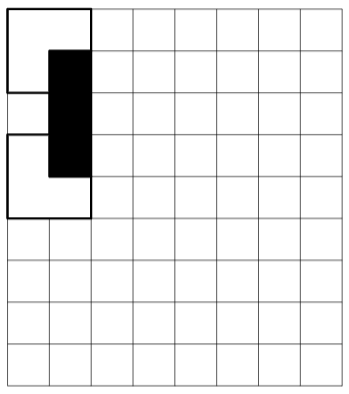
\includegraphics[width=.15\textwidth]{images/B(8, 9).png} % images/그림파일 이름
    \caption{bad pair of $9\times 8$ deficient tile} % 그림 캡션
    \label{fig:my_label} % 그림의 위치를 지시할 때 쓰는 label
\end{figure}

\begin{definition}
정의란 무엇일까? \citep{aanjaneya2009tromino, golomb2021polyominoes, nitica2017tilings} % 참고문헌 표기
\end{definition}

\jiwon[3-4] % 더미 텍스트

\begin{theorem}\label{thm:what}
    정리란 무엇일까?
\end{theorem}



\subsection{그림 삽입 방법}

%--------- 그림 삽입 방법 설명(내용을 확인 한 후에, 삭제하세요).
아래에서는 그림을 삽입하는 방법을 안내한다. 크게 두 가지 방법이 있다.
\begin{enumerate}[(a)]
    \item 그림 파일을 images 폴더에 업로드 한 후, 그 파일을 넣는 방식.
    \item 텍을 이용하여 직접 그림을 그리는 방식.
\end{enumerate}
그러나, 어느 방식이든, 그림의 위치를 \TeX에게 맡기려면, figure 환경을 이용해야한다. 또 하나의 팁을 주자면, 그림파일을 미리 준비하지 않았더라도, \TeX이 갖고 있는 예시그림을 이용하여 그림의 위치를 미리 어느 정도 살펴볼 수 있다는 것이다. 

다음 예시는 \TeX이 갖고 있는 그림예제를 이용하여 그림을 삽입해 본 것이다.

\begin{figure}[!ht]
    \centering
    \includegraphics[width=.4\textwidth]{example-image} % images/그림파일 이름
    \caption{이 그림의 캡션은?!}
    \label{fig:my_fig_label}
\end{figure}


다음 예시는 텍을 이용하여 직접 그림을 그리는 예이다.
\begin{center}
 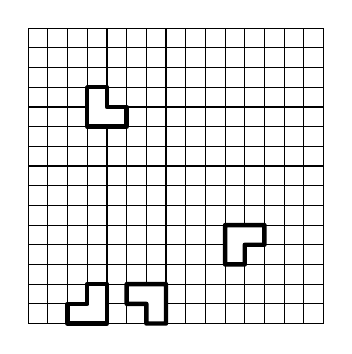
\begin{tikzpicture}[scale=.5]
 	\checkerboard{15}{15} 	% 그리드를 그리는 명령 \checkerboard{"가로칸 수"}{"세로칸 수"}
	\LtrominoNE{3}{10}
	\LtrominoNW{4}{0}
	\LtrominoSW{6}{1}
	\LtrominoSE{10}{5}
 \end{tikzpicture}
\end{center}
이 그림은 figure 환경에 그린 것이 아니기 때문에, 별도의 캡션이 달려있지는 않다. 그림 \ref{fig:my_label}\을 참고하라.

%------------ 그림 삽입 방법 설명 끝. 

\subsection{표 삽입 방법}
한편 표를 삽입하는 방법은 그림을 삽입하는 방법과 거의 동일하다. figure 환경을 table환경으로 바꾸기만 하면 된다. 표를 텍에서 집접 그리는 것은 좀 번거로울 수 있다. 불편하다면, 다른 표 작성도구로 표를 만든 다음 이를 그림으로 집어 넣되 다만 table 환경을 이용하여 삽입하면 캡션이 자연스럽게 잘 붙을 것이다.

\begin{table}[!ht]
    \centering
    % 표를 만드는 가장 좋은 환경은 tblr 환경이다. (tabularray페키지 필요) 그리고 https://www.tablesgenerator.com/ 를 이용하면 아주 편리하다.
    \caption{이 표의 캡션은?!}
    \label{tab:my_label}
    \begin{tblr}{|l|l|l|}
        \hline
          & 위치 & 장소 \\ \hline
        1 &    &    \\ \hline
        2 &    &    \\ \hline
        3 &    &    \\ \hline
    \end{tblr}
\end{table}



\subsection{수식 입력 방법}
이번에는 수식을 작성하는 몇 가지 예를 살펴보자. 수식은 크게 두 가지 모드로 작성한다.
\begin{itemize}
    \item 행중수식: 문단을 바꾸지 않고 쓰는 수식
    \item 행간수식: 문단을 별도로 두어 별도의 행에 쓰는 수식
\end{itemize}
구체적인 몇 가지 예를 통해서 수식을 입력하는 방법을 살펴보자.

%----------- 수식 작성 예졔
\begin{itemize}
    \item 아래첨자.

아래첨자는, 예를 들어, 이렇게 쓰면 된다. $A_{b+c}$. 여기서 $A_a+b$와 비교해보아라. 아! 그리고 곱하기는 $a\times b$와 같이 쓴다.
\item 최대정수함수 기호. 

국제표준(?) 방식으로 써보자. $\lfloor x\rfloor$로 쓰면 된다. 최대정수함수를 비롯한, 소위, 괄호류(?)는 괄호 안에 들어 있는 수식의 크기에 맞게 괄호의 크기가 바뀌어야겠죠! 아래의 두 식을 비료해 보세요.
\[ \lfloor \frac{\pi^2}{6}\rfloor \]
으, 못생긴 식이다.
\[ \left\lfloor \frac{\pi^2}{6}\right\rfloor \]
그렇다. $\left( \frac{1}{2} \right)$와 같이 쓰면 된다.

\item 분수 표기는 $\frac{2}{3}$과 같이 쓰면 된다. 행간수식을 이용해서 분수를 표기하면 
\[ \frac{df}{dt}=\frac{df}{ds}\frac{ds}{dt} \]
와 같이 분수의 크기가 커진다.


\item 부등호는 알다시피 $1\leq 3\leq 5 \geq 2$.

\item 합동식.

몇 가지 방법이 있다. 우선 세 줄짜리 등호는 $\equiv$ 이렇게. 아래에서는 여러 줄에 걸친 수식을 쓰는 법도 함께 보자. 소스에 등장하는 \& 는 수식을 정렬하는 도구로 이해하면 된다. 줄바꿈은 백슬래시 두 개!
\begin{align*}
a & \equiv b \mod{p} \\
a & \equiv b \pmod{p}
\end{align*}
음, 두 번째 방법으로 쓰면 되겠구나.
\end{itemize}
%---------- 수식 작성 예제 끝.



\section{결론} 
\jiwon[4] % 더미 텍스트








%%\citep{}; 내용에서 논문 참조할 때 

%\nocite{defant2020counting, egge2004132, goodrich2012sorting, park2013avoiding, ulfarsson2011describing}


\section{참고문헌}
\printbibliography[heading=none]



%%%%%%%%% 영문 초록이 필요하다면, 아래 주석 처리를 취소하라.
% \newpage
% \begin{abstract}
% \begin{spacing}{1}
% %%% 영문초록 입력
% % 내용 작성 시 아래 \lipsum[1] 을 삭제(혹은 주석처리) 후 입력하세요.
\lipsum[1] % 더미 텍스트 

% %%% 영문초록 입력 끝
% \vskip5pt
% \noindent {\bfseries Keywords:}\ \mykeywords
% \end{spacing}
% \end{abstract}
%%%%%%%%%%%%% 영문 초록 부분 끝
\end{document}

